% Day 3: Cryptographic Foundations -- Building Trust Without Institutions
% Digital Finance Introduction
\documentclass[11pt,aspectratio=169]{beamer}
\usetheme{Madrid}

% ======================= PACKAGES =======================
\usepackage{graphicx}
\usepackage{booktabs}
\usepackage{adjustbox}
\usepackage{multicol}
\usepackage{amsmath}
\usepackage{amssymb}
\usepackage{tikz}
\usetikzlibrary{arrows,shapes,positioning,shadows,trees}
\usepackage{listings}
\usepackage{xcolor}

% ======================= COLOR DEFINITIONS =======================
% Primary color scheme: Blue/Teal for Digital Finance
\definecolor{dfblue}{RGB}{0,102,204}
\definecolor{dfteal}{RGB}{0,153,153}
\definecolor{dfcyan}{RGB}{51,187,204}
\definecolor{dflightblue}{RGB}{153,204,255}
\definecolor{dflightblue2}{RGB}{173,214,255}
\definecolor{dflightblue3}{RGB}{193,224,255}
\definecolor{dflightblue4}{RGB}{213,234,255}

% Accent colors for finance applications
\definecolor{dfgreen}{RGB}{44, 160, 44}
\definecolor{dfred}{RGB}{214, 39, 40}
\definecolor{dforange}{RGB}{255, 127, 14}
\definecolor{dfgray}{RGB}{127, 127, 127}

% Utility colors
\definecolor{lightgray}{RGB}{240, 240, 240}
\definecolor{midgray}{RGB}{180, 180, 180}
\definecolor{codebg}{RGB}{245, 245, 245}

% ======================= THEME CUSTOMIZATION =======================
% Apply Digital Finance color scheme to Madrid theme
\setbeamercolor{palette primary}{bg=dflightblue3,fg=dfblue}
\setbeamercolor{palette secondary}{bg=dflightblue2,fg=dfblue}
\setbeamercolor{palette tertiary}{bg=dfteal,fg=white}
\setbeamercolor{palette quaternary}{bg=dfblue,fg=white}

\setbeamercolor{structure}{fg=dfblue}
\setbeamercolor{section in toc}{fg=dfblue}
\setbeamercolor{subsection in toc}{fg=dfteal}
\setbeamercolor{title}{fg=dfblue}
\setbeamercolor{frametitle}{fg=dfblue,bg=dflightblue3}
\setbeamercolor{block title}{bg=dflightblue2,fg=dfblue}
\setbeamercolor{block body}{bg=dflightblue4,fg=black}

% Remove navigation symbols for cleaner look
\setbeamertemplate{navigation symbols}{}

% Clean itemize/enumerate
\setbeamertemplate{itemize items}[circle]
\setbeamertemplate{enumerate items}[default]

% Margins for readability
\setbeamersize{text margin left=8mm,text margin right=8mm}

% ======================= LISTINGS CONFIGURATION =======================
% Python code style
\lstdefinestyle{pythonstyle}{
    language=Python,
    basicstyle=\ttfamily\footnotesize,
    keywordstyle=\color{dfblue}\bfseries,
    stringstyle=\color{dforange},
    commentstyle=\color{dfgray}\itshape,
    numberstyle=\tiny\color{dfgray},
    numbers=left,
    numbersep=5pt,
    backgroundcolor=\color{codebg},
    showspaces=false,
    showstringspaces=false,
    showtabs=false,
    frame=single,
    rulecolor=\color{midgray},
    tabsize=4,
    captionpos=b,
    breaklines=true,
    breakatwhitespace=false,
    escapeinside={(*@}{@*)},
    xleftmargin=10pt,
    xrightmargin=10pt
}

% Solidity code style
\lstdefinestyle{soliditystyle}{
    language=Java, % closest approximation
    basicstyle=\ttfamily\footnotesize,
    keywordstyle=\color{dfteal}\bfseries,
    stringstyle=\color{dforange},
    commentstyle=\color{dfgray}\itshape,
    numberstyle=\tiny\color{dfgray},
    numbers=left,
    numbersep=5pt,
    backgroundcolor=\color{codebg},
    showspaces=false,
    showstringspaces=false,
    showtabs=false,
    frame=single,
    rulecolor=\color{midgray},
    tabsize=2,
    captionpos=b,
    breaklines=true,
    breakatwhitespace=false,
    escapeinside={(*@}{@*)},
    xleftmargin=10pt,
    xrightmargin=10pt,
    morekeywords={pragma, contract, function, returns, public, private, view, pure, payable, address, uint256, mapping, event, modifier}
}

% Inline code command
\newcommand{\code}[1]{\texttt{\color{dfblue}#1}}

% ======================= CUSTOM COMMANDS =======================
% Bottom annotation (Madrid-style)
\newcommand{\bottomnote}[1]{%
\vfill
\vspace{-2mm}
\textcolor{dflightblue2}{\rule{\textwidth}{0.4pt}}
\vspace{1mm}
\footnotesize
\textbf{#1}
}

% Compact list spacing
\newcommand{\compactlist}{%
\setlength{\itemsep}{0pt}%
\setlength{\parskip}{0pt}%
\setlength{\parsep}{0pt}%
}

% Chart placeholder
\newcommand{\chartplaceholder}[2][5cm]{%
\begin{center}
\begin{adjustbox}{max width=0.95\textwidth, max height=#1}
\framebox[\textwidth][c]{%
\rule{0pt}{#1}%
\textcolor{midgray}{[#2]}%
}
\end{adjustbox}
\end{center}
}

% ======================= FINANCE NOTATION MACROS =======================
% Probability and statistics
\newcommand{\E}{\mathbb{E}} % Expected value
\newcommand{\Var}{\mathrm{Var}} % Variance
\newcommand{\Cov}{\mathrm{Cov}} % Covariance
\newcommand{\Prob}{\mathbb{P}} % Probability

% Distributions
\newcommand{\Normal}{\mathcal{N}} % Normal distribution
\newcommand{\Uniform}{\mathcal{U}} % Uniform distribution

% Returns and prices
\newcommand{\Ret}{R} % Return
\newcommand{\LogRet}{r} % Log return
\newcommand{\Price}{S} % Price/Stock price
\newcommand{\Strike}{K} % Strike price

% Options and derivatives
\newcommand{\CallPrice}{C} % Call option price
\newcommand{\PutPrice}{P} % Put option price
\newcommand{\Greeks}[1]{\mathit{#1}} % Greek letters

% Risk measures
\newcommand{\VaR}{\mathrm{VaR}} % Value at Risk
\newcommand{\CVaR}{\mathrm{CVaR}} % Conditional VaR
\newcommand{\Sharpe}{\mathrm{SR}} % Sharpe Ratio

% Time series
\newcommand{\AR}{\mathrm{AR}} % Autoregressive
\newcommand{\MA}{\mathrm{MA}} % Moving average
\newcommand{\GARCH}{\mathrm{GARCH}} % GARCH

% Blockchain/Crypto
\newcommand{\Hash}{\mathrm{Hash}} % Hash function
\newcommand{\Block}{\mathcal{B}} % Block
\newcommand{\Chain}{\mathcal{C}} % Chain

% Real numbers, integers
\newcommand{\R}{\mathbb{R}}
\newcommand{\Z}{\mathbb{Z}}
\newcommand{\N}{\mathbb{N}}

% ======================= TIKZ STYLES =======================
% Styles for finance-related diagrams
\tikzstyle{process} = [rectangle, minimum width=3cm, minimum height=1cm, text centered, draw=dfblue, fill=dflightblue4, thick]
\tikzstyle{decision} = [diamond, minimum width=3cm, minimum height=1cm, text centered, draw=dfteal, fill=dflightblue4, thick]
\tikzstyle{arrow} = [thick,->,>=stealth,color=dfblue]
\tikzstyle{blockchain} = [rectangle, rounded corners, minimum width=2.5cm, minimum height=1cm, text centered, draw=dfteal, fill=dflightblue3, thick]
\tikzstyle{transaction} = [circle, minimum size=0.8cm, text centered, draw=dforange, fill=dflightblue4, thick]

% ======================= FOOTER TEMPLATE =======================
\setbeamertemplate{footline}{
    \hbox{\begin{beamercolorbox}[wd=\paperwidth,ht=2.5ex,dp=1ex,leftskip=.5em,rightskip=.5em]{author in head/foot}
    \tiny
    \textbf{Digital Finance} \hfill
    Joerg Osterrieder \hfill
    \insertdate \hfill
    Page \insertframenumber{} / \inserttotalframenumber
    \end{beamercolorbox}}
}

% ======================= SECTION DIVIDER TEMPLATE =======================
\AtBeginSection[]{
\begin{frame}[plain]
\vfill
\centering
\begin{beamercolorbox}[sep=12pt,center]{title}
\usebeamerfont{title}\LARGE\insertsection\par
\end{beamercolorbox}
\vfill
\end{frame}
}


% ======================= DOCUMENT INFO =======================
\title[Day 3: Cryptographic Foundations]{Day 3: Cryptographic Foundations\\Building Trust Without Institutions}
\subtitle{Digital Finance Introduction}
\author{Prof. Dr. Joerg Osterrieder}
\institute{Digital Finance}
\date{2025}

% Additional TikZ libraries for this day
\usetikzlibrary{chains,calc,decorations.pathreplacing,fit,backgrounds}

% Custom styles for cryptography diagrams
\tikzstyle{hashbox} = [rectangle, rounded corners, minimum width=2cm, minimum height=0.8cm, text centered, draw=dfteal, fill=dflightblue3, thick, font=\footnotesize]
\tikzstyle{databox} = [rectangle, minimum width=2.5cm, minimum height=0.6cm, text centered, draw=dfblue, fill=dflightblue4, thick, font=\footnotesize]
\tikzstyle{keybox} = [rectangle, rounded corners, minimum width=2cm, minimum height=0.6cm, text centered, draw=dforange, fill=dflightblue4, thick, font=\footnotesize]
\tikzstyle{blocknode} = [rectangle, rounded corners, minimum width=3cm, minimum height=2cm, text centered, draw=dfteal, fill=dflightblue3, thick]
\tikzstyle{walletbox} = [rectangle, rounded corners, minimum width=2.5cm, minimum height=1cm, text centered, draw=dfgreen, fill=dflightblue4, thick]

\begin{document}

% ======================= TITLE SLIDE =======================
\begin{frame}[plain]
\titlepage
\end{frame}

% ======================= DAY OVERVIEW =======================
\begin{frame}{Day 3 Overview}
\begin{columns}[T]
\begin{column}{0.48\textwidth}
\textbf{Morning Sessions}
\begin{enumerate}
\item \textbf{3.1 Cryptographic Building Blocks}\\
{\small Hashing, Keys, Digital Signatures}
\vspace{2mm}
\item \textbf{3.2 Blockchain Mechanics}\\
{\small Consensus, Blocks, Trilemma}
\end{enumerate}
\end{column}
\begin{column}{0.48\textwidth}
\textbf{Afternoon Sessions}
\begin{enumerate}
\setcounter{enumi}{2}
\item \textbf{3.3 Wallets \& Transactions}\\
{\small User Experience Gap}
\vspace{2mm}
\item \textbf{3.4 Bitcoin vs. Ethereum}\\
{\small Two Design Philosophies}
\end{enumerate}
\end{column}
\end{columns}

\vspace{5mm}
\begin{center}
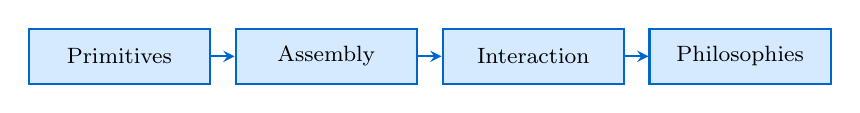
\begin{tikzpicture}[node distance=0.3cm]
\node[process, minimum width=2.3cm, minimum height=0.7cm] (n1) {\footnotesize Primitives};
\node[process, minimum width=2.3cm, minimum height=0.7cm, right=of n1] (n2) {\footnotesize Assembly};
\node[process, minimum width=2.3cm, minimum height=0.7cm, right=of n2] (n3) {\footnotesize Interaction};
\node[process, minimum width=2.3cm, minimum height=0.7cm, right=of n3] (n4) {\footnotesize Philosophies};
\draw[arrow] (n1) -- (n2);
\draw[arrow] (n2) -- (n3);
\draw[arrow] (n3) -- (n4);
\end{tikzpicture}
\end{center}

\bottomnote{Day Arc: From smallest building blocks to highest-level design philosophy}
\end{frame}

% ======================= TABLE OF CONTENTS =======================
\begin{frame}{Agenda}
\tableofcontents
\end{frame}

% ======================= PEDAGOGICAL BRIDGE =======================
\begin{frame}{Connecting to Day 1: The Trust Problem}
\textbf{Remember from Day 1:}
\begin{itemize}
\item Financial systems require \textbf{trust} between parties
\item Traditional solution: Trusted intermediaries (banks, clearinghouses)
\item Digital alternative: Mathematical/cryptographic guarantees
\end{itemize}

\vspace{3mm}
\textbf{Today we explore HOW cryptography provides trust:}
\begin{itemize}
\item Hash functions $\rightarrow$ Data integrity verification
\item Digital signatures $\rightarrow$ Identity and authorization
\item Blockchain $\rightarrow$ Tamper-evident, distributed ledgers
\end{itemize}

\vspace{3mm}
\textit{Note: This material is more technical than Days 1-2. Take your time with the concepts.}
\end{frame}

\begin{frame}{Key Technical Terms}
\textbf{Definitions you'll encounter today:}

\begin{description}
\item[Turing-complete] A system that can compute anything computable (like a general-purpose computer). Ethereum is Turing-complete; Bitcoin is not.
\item[Byzantine fault tolerant] A system that works correctly even when some participants are malicious or fail. Named after the ``Byzantine Generals Problem.''
\item[Nonce] ``Number used once'' -- a value that changes to produce different hash outputs.
\item[Gas] Ethereum's unit for measuring computational work. More complex operations cost more gas.
\end{description}

\vspace{3mm}
\textit{Don't worry if these feel abstract now---they'll make more sense as we work through examples.}
\end{frame}

% =======================================================================
% SECTION 3.1: CRYPTOGRAPHIC BUILDING BLOCKS
% =======================================================================
\section{3.1 Cryptographic Building Blocks}

\begin{frame}{The Trust Problem in Digital Systems}
\begin{columns}[T]
\begin{column}{0.5\textwidth}
\textbf{Traditional Trust Model}
\begin{itemize}
\item Banks verify your identity
\item Courts enforce contracts
\item Governments back currency
\item Intermediaries everywhere
\end{itemize}
\vspace{3mm}
\textcolor{dfred}{Problem: Single points of failure}
\end{column}
\begin{column}{0.5\textwidth}
\textbf{Cryptographic Trust Model}
\begin{itemize}
\item Mathematics verifies identity
\item Code enforces agreements
\item Network backs value
\item Trust is distributed
\end{itemize}
\vspace{3mm}
\textcolor{dfgreen}{Solution: Trust through verification}
\end{column}
\end{columns}

\vspace{5mm}
\begin{center}
\fbox{\parbox{0.8\textwidth}{\centering
\textbf{Key Insight:} Cryptography lets us replace ``trust me'' with ``verify this''
}}
\end{center}
\end{frame}

\begin{frame}{Three Cryptographic Primitives}
\begin{center}
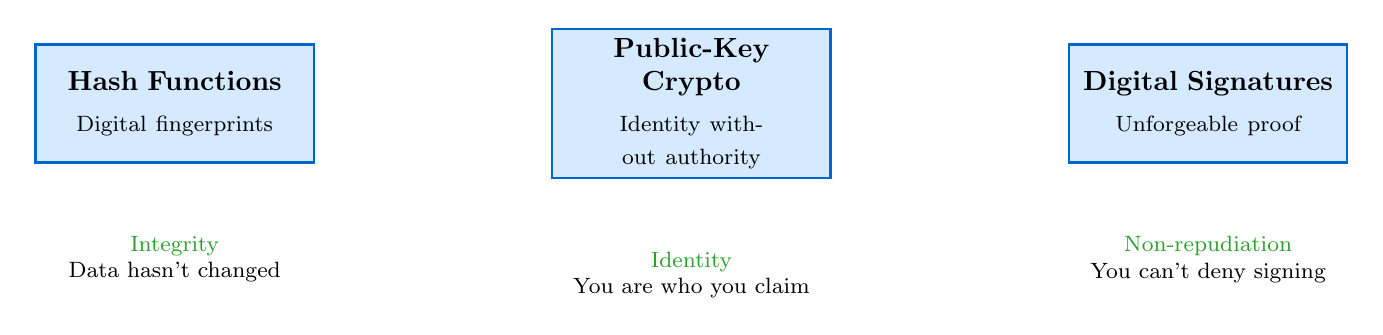
\begin{tikzpicture}[node distance=3cm]
% Three main boxes
\node[process, minimum width=3.5cm, minimum height=1.5cm, text width=3.3cm, align=center] (hash) {
\textbf{Hash Functions}\\[1mm]
\footnotesize Digital fingerprints
};
\node[process, minimum width=3.5cm, minimum height=1.5cm, text width=3.3cm, align=center, right=of hash] (keys) {
\textbf{Public-Key Crypto}\\[1mm]
\footnotesize Identity without authority
};
\node[process, minimum width=3.5cm, minimum height=1.5cm, text width=3.3cm, align=center, right=of keys] (sigs) {
\textbf{Digital Signatures}\\[1mm]
\footnotesize Unforgeable proof
};

% What they guarantee
\node[below=0.8cm of hash, text width=3.5cm, align=center, font=\footnotesize] {
\textcolor{dfgreen}{Integrity}\\
Data hasn't changed
};
\node[below=0.8cm of keys, text width=3.5cm, align=center, font=\footnotesize] {
\textcolor{dfgreen}{Identity}\\
You are who you claim
};
\node[below=0.8cm of sigs, text width=3.5cm, align=center, font=\footnotesize] {
\textcolor{dfgreen}{Non-repudiation}\\
You can't deny signing
};
\end{tikzpicture}
\end{center}

\vspace{3mm}
\textbf{Focus:} What these tools \textit{guarantee}, not how the math works

\bottomnote{These three primitives are the atoms of decentralized trust}
\end{frame}

% --- HASH FUNCTIONS ---
\begin{frame}{Hash Functions: Digital Fingerprints}
\begin{center}
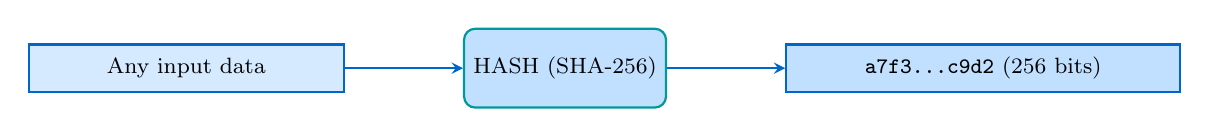
\begin{tikzpicture}
% Input
\node[databox, minimum width=4cm] (input) {Any input data};
% Hash function
\node[hashbox, right=1.5cm of input, minimum width=2.5cm, minimum height=1cm] (hash) {HASH (SHA-256)};
% Output
\node[databox, right=1.5cm of hash, minimum width=5cm, fill=dflightblue3] (output) {\texttt{a7f3...c9d2} (256 bits)};

\draw[arrow] (input) -- (hash);
\draw[arrow] (hash) -- (output);
\end{tikzpicture}
\end{center}

\vspace{5mm}
\begin{tabular}{ll}
\textcolor{dfblue}{\textbf{Deterministic:}} & Same input $\rightarrow$ same output, always\\[2mm]
\textcolor{dfblue}{\textbf{One-way:}} & Cannot reverse to find input\\[2mm]
\textcolor{dfblue}{\textbf{Collision-resistant:}} & Practically impossible to find two inputs with same hash\\[2mm]
\textcolor{dfblue}{\textbf{Avalanche effect:}} & Tiny change $\rightarrow$ completely different output\\
\end{tabular}
\end{frame}

\begin{frame}{Hash Function Visualization: The Avalanche Effect}
\begin{center}
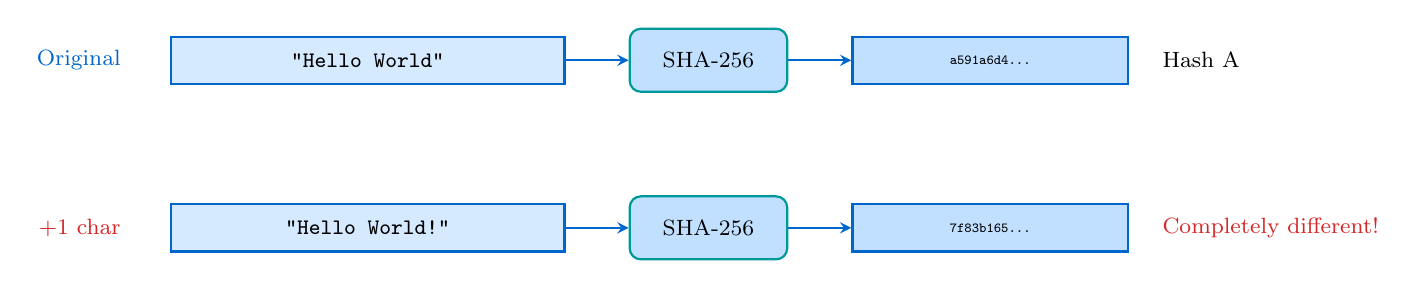
\begin{tikzpicture}[node distance=0.8cm]
% Example 1
\node[databox, minimum width=5cm] (in1) {\texttt{"Hello World"}};
\node[hashbox, right=0.8cm of in1, minimum width=2cm] (h1) {SHA-256};
\node[databox, right=0.8cm of h1, minimum width=3.5cm, fill=dflightblue3, font=\tiny\ttfamily] (out1) {a591a6d4...};
\draw[arrow] (in1) -- (h1);
\draw[arrow] (h1) -- (out1);

% Example 2 - tiny change
\node[databox, minimum width=5cm, below=1.5cm of in1] (in2) {\texttt{"Hello World!"}};
\node[hashbox, right=0.8cm of in2, minimum width=2cm] (h2) {SHA-256};
\node[databox, right=0.8cm of h2, minimum width=3.5cm, fill=dflightblue3, font=\tiny\ttfamily] (out2) {7f83b165...};
\draw[arrow] (in2) -- (h2);
\draw[arrow] (h2) -- (out2);

% Annotations
\node[left=0.5cm of in1, font=\footnotesize, text=dfblue] {Original};
\node[left=0.5cm of in2, font=\footnotesize, text=dfred] {+1 char};
\node[right=0.3cm of out1, font=\footnotesize] {Hash A};
\node[right=0.3cm of out2, font=\footnotesize, text=dfred] {Completely different!};
\end{tikzpicture}
\end{center}

\vspace{5mm}
\textbf{Why this matters for blockchain:}
\begin{itemize}
\item Change one transaction $\rightarrow$ entire block hash changes
\item This change cascades through all subsequent blocks
\item Tampering becomes immediately detectable
\end{itemize}
\end{frame}

\begin{frame}{What Hash Functions Guarantee}
\begin{columns}[T]
\begin{column}{0.55\textwidth}
\textbf{Use Cases in Blockchain}
\begin{itemize}\compactlist
\item \textbf{Data integrity:} Verify nothing changed
\item \textbf{Block linking:} Each block contains hash of previous
\item \textbf{Transaction IDs:} Unique identifier for every transaction
\item \textbf{Mining puzzles:} Finding hashes with specific properties
\item \textbf{Merkle trees:} Efficiently verify large data sets
\end{itemize}
\end{column}
\begin{column}{0.42\textwidth}
\begin{center}
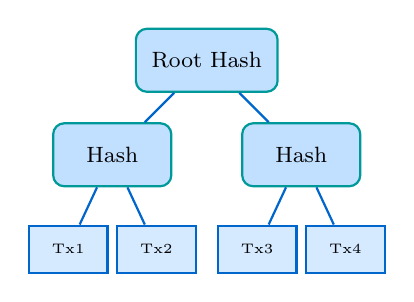
\begin{tikzpicture}[scale=0.8]
% Merkle tree
\node[hashbox, minimum width=1.8cm] (root) at (0,3) {Root Hash};
\node[hashbox, minimum width=1.5cm] (h1) at (-1.5,1.5) {Hash};
\node[hashbox, minimum width=1.5cm] (h2) at (1.5,1.5) {Hash};
\node[databox, minimum width=1cm, font=\tiny] (t1) at (-2.2,0) {Tx1};
\node[databox, minimum width=1cm, font=\tiny] (t2) at (-0.8,0) {Tx2};
\node[databox, minimum width=1cm, font=\tiny] (t3) at (0.8,0) {Tx3};
\node[databox, minimum width=1cm, font=\tiny] (t4) at (2.2,0) {Tx4};

\draw[thick, dfblue] (t1) -- (h1);
\draw[thick, dfblue] (t2) -- (h1);
\draw[thick, dfblue] (t3) -- (h2);
\draw[thick, dfblue] (t4) -- (h2);
\draw[thick, dfblue] (h1) -- (root);
\draw[thick, dfblue] (h2) -- (root);
\end{tikzpicture}

\footnotesize\textbf{Merkle Tree}\\
Verify any transaction with $O(\log n)$ hashes
\end{center}
\end{column}
\end{columns}

\vspace{3mm}
\begin{block}{The Guarantee}
If two hashes match, the data is identical (with overwhelming probability).
\end{block}
\end{frame}

% --- PUBLIC-KEY CRYPTOGRAPHY ---
\begin{frame}{Public-Key Cryptography: Identity Without Authority}
\begin{center}
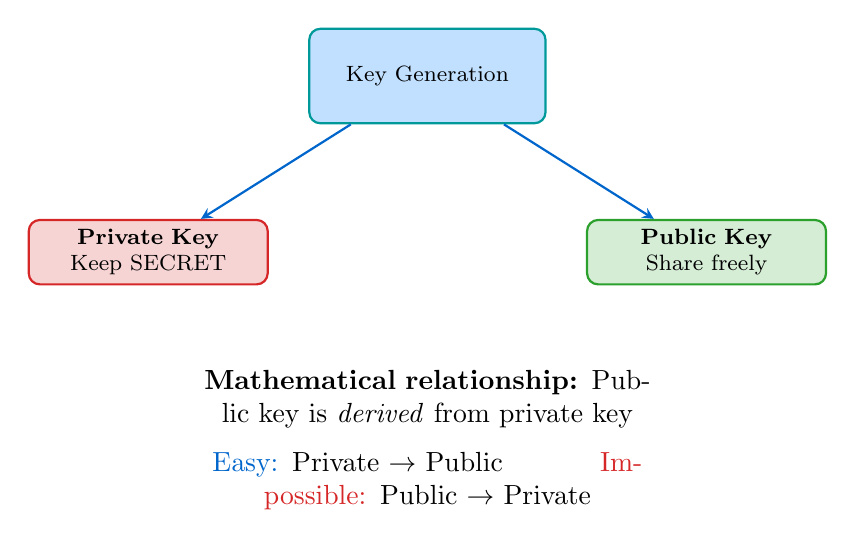
\begin{tikzpicture}[node distance=1cm]
% Key generation
\node[hashbox, minimum width=3cm, minimum height=1.2cm] (gen) {Key Generation};

% Private key
\node[keybox, below left=1.2cm and 0.5cm of gen, fill=dfred!20, draw=dfred, minimum width=3cm, text width=2.8cm, align=center] (priv) {
\textbf{Private Key}\\
\footnotesize Keep SECRET
};

% Public key
\node[keybox, below right=1.2cm and 0.5cm of gen, fill=dfgreen!20, draw=dfgreen, minimum width=3cm, text width=2.8cm, align=center] (pub) {
\textbf{Public Key}\\
\footnotesize Share freely
};

\draw[arrow] (gen) -- (priv);
\draw[arrow] (gen) -- (pub);

% Relationship
\node[below=3cm of gen, text width=9cm, align=center] {
\textbf{Mathematical relationship:} Public key is \textit{derived} from private key\\[2mm]
\textcolor{dfblue}{Easy:} Private $\rightarrow$ Public \hspace{1cm}
\textcolor{dfred}{Impossible:} Public $\rightarrow$ Private
};
\end{tikzpicture}
\end{center}
\end{frame}

\begin{frame}{Public-Key Cryptography: How It Works}
\begin{center}
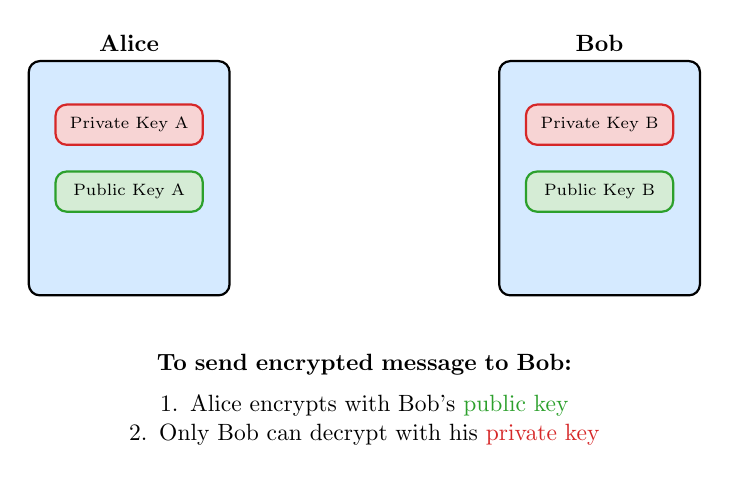
\begin{tikzpicture}[node distance=0.5cm, scale=0.85, transform shape]
% Alice
\node[draw, thick, rounded corners, minimum width=3cm, minimum height=3.5cm, fill=dflightblue4] (alice) {};
\node[above=0mm of alice.north, font=\bfseries] {Alice};
\node[keybox, fill=dfred!20, draw=dfred, minimum width=2.2cm, font=\scriptsize] at ($(alice.center) + (0,0.8)$) {Private Key A};
\node[keybox, fill=dfgreen!20, draw=dfgreen, minimum width=2.2cm, font=\scriptsize] at ($(alice.center) + (0,-0.2)$) {Public Key A};

% Bob
\node[draw, thick, rounded corners, minimum width=3cm, minimum height=3.5cm, fill=dflightblue4, right=4cm of alice] (bob) {};
\node[above=0mm of bob.north, font=\bfseries] {Bob};
\node[keybox, fill=dfred!20, draw=dfred, minimum width=2.2cm, font=\scriptsize] at ($(bob.center) + (0,0.8)$) {Private Key B};
\node[keybox, fill=dfgreen!20, draw=dfgreen, minimum width=2.2cm, font=\scriptsize] at ($(bob.center) + (0,-0.2)$) (bpub) {Public Key B};

% Message flow
\node[below=2.5cm of $(alice)!0.5!(bob)$, text width=8cm, align=center] {
\textbf{To send encrypted message to Bob:}\\[2mm]
1. Alice encrypts with Bob's \textcolor{dfgreen}{public key}\\
2. Only Bob can decrypt with his \textcolor{dfred}{private key}
};
\end{tikzpicture}
\end{center}

\vspace{2mm}
\textbf{Key insight:} Only the person with the private key can decrypt
\end{frame}

\begin{frame}{From Public Key to Blockchain Address}
\begin{center}
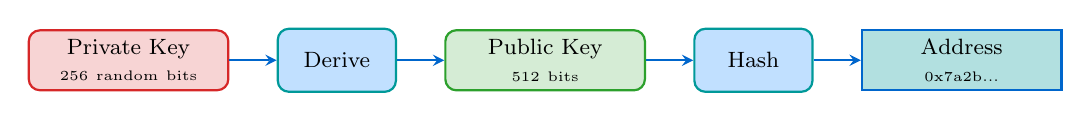
\begin{tikzpicture}[node distance=0.4cm]
% Flow
\node[keybox, fill=dfred!20, draw=dfred, minimum width=2.5cm, text width=2.3cm, align=center] (priv) {Private Key\\{\tiny 256 random bits}};
\node[hashbox, right=0.6cm of priv, minimum width=1.5cm] (derive) {Derive};
\node[keybox, fill=dfgreen!20, draw=dfgreen, minimum width=2.5cm, text width=2.3cm, align=center, right=0.6cm of derive] (pub) {Public Key\\{\tiny 512 bits}};
\node[hashbox, right=0.6cm of pub, minimum width=1.5cm] (hash) {Hash};
\node[databox, fill=dfteal!30, minimum width=2.5cm, text width=2.3cm, align=center, right=0.6cm of hash] (addr) {Address\\{\tiny 0x7a2b...}};

\draw[arrow] (priv) -- (derive);
\draw[arrow] (derive) -- (pub);
\draw[arrow] (pub) -- (hash);
\draw[arrow] (hash) -- (addr);
\end{tikzpicture}
\end{center}

\vspace{5mm}
\begin{columns}[T]
\begin{column}{0.48\textwidth}
\textbf{What You Control}
\begin{itemize}
\item Private key = your identity
\item Whoever has it controls the funds
\item \textcolor{dfred}{Lose it = lose everything}
\item \textcolor{dfred}{Share it = share everything}
\end{itemize}
\end{column}
\begin{column}{0.48\textwidth}
\textbf{What You Share}
\begin{itemize}
\item Address = your ``account number''
\item Safe to share publicly
\item Used to receive payments
\item Cannot derive private key from it
\end{itemize}
\end{column}
\end{columns}

\bottomnote{``Not your keys, not your coins'' -- a fundamental principle of crypto}
\end{frame}

% --- DIGITAL SIGNATURES ---
\begin{frame}{Digital Signatures: Unforgeable Proof}
\begin{center}
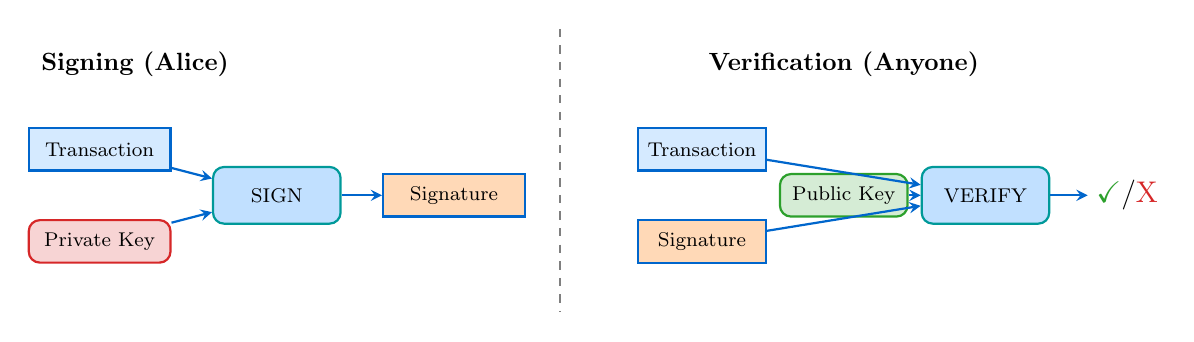
\begin{tikzpicture}[node distance=0.5cm, scale=0.9, transform shape]
% Signing process
\node[font=\bfseries] at (-4.5, 2) {Signing (Alice)};

\node[databox, minimum width=2cm] (msg) at (-5,0.8) {Transaction};
\node[keybox, fill=dfred!20, draw=dfred, minimum width=2cm] (key) at (-5,-0.5) {Private Key};
\node[hashbox, minimum width=1.8cm] (sign) at (-2.5,0.15) {SIGN};
\node[databox, fill=dforange!30, minimum width=2cm] (sig) at (0,0.15) {Signature};

\draw[arrow] (msg) -- (sign);
\draw[arrow] (key) -- (sign);
\draw[arrow] (sign) -- (sig);

% Verification process
\node[font=\bfseries] at (5.5, 2) {Verification (Anyone)};

\node[databox, minimum width=1.8cm] (msg2) at (3.5,0.8) {Transaction};
\node[databox, fill=dforange!30, minimum width=1.8cm] (sig2) at (3.5,-0.5) {Signature};
\node[keybox, fill=dfgreen!20, draw=dfgreen, minimum width=1.8cm] (pub) at (5.5,0.15) {Public Key};
\node[hashbox, minimum width=1.8cm] (verify) at (7.5,0.15) {VERIFY};
\node[font=\large] (result) at (9.5,0.15) {\textcolor{dfgreen}{\checkmark}/\textcolor{dfred}{X}};

\draw[arrow] (msg2) -- (verify);
\draw[arrow] (sig2) -- (verify);
\draw[arrow] (pub) -- (verify);
\draw[arrow] (verify) -- (result);

% Divider
\draw[thick, dashed, dfgray] (1.5,2.5) -- (1.5,-1.5);
\end{tikzpicture}
\end{center}

\vspace{3mm}
\textbf{What Digital Signatures Guarantee:}
\begin{itemize}
\item \textbf{Authentication:} Only private key holder could create this signature
\item \textbf{Integrity:} The message hasn't been altered
\item \textbf{Non-repudiation:} Signer cannot deny having signed
\end{itemize}
\end{frame}

\begin{frame}{Digital Signatures in Blockchain}
Every blockchain transaction includes a digital signature proving authorization:

\vspace{3mm}
\begin{center}
\begin{tabular}{|l|l|}
\hline
\textbf{Field} & \textbf{Value} \\
\hline
From & 0x7a2b...9f3c \\
To & 0x9c4d...e8f2 \\
Value & 1.5 ETH \\
Nonce & 42 \\
Gas Limit & 21,000 \\
Gas Price & 50 gwei \\
\textbf{Signature} & \textit{v, r, s (proves authorization)} \\
\hline
\end{tabular}
\end{center}

\vspace{5mm}
\textbf{How it works in practice:}
\begin{enumerate}
\item Alice creates transaction: ``Send 1.5 ETH to Bob''
\item Alice signs with her private key
\item Network verifies signature using Alice's public key
\item If valid: transaction is processed. If invalid: rejected
\end{enumerate}
\end{frame}

\begin{frame}{Summary: The Cryptographic Trust Stack}
\begin{center}
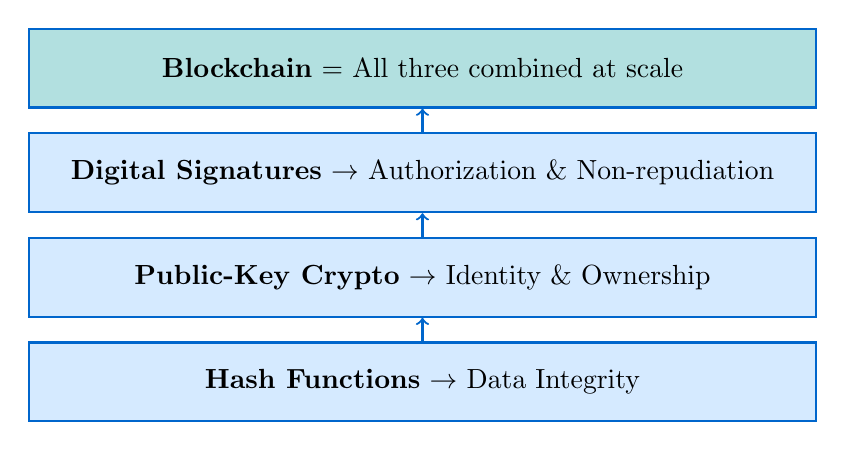
\begin{tikzpicture}[node distance=0.3cm]
% Stack of guarantees
\node[process, minimum width=10cm, minimum height=1cm] (l1) {
\textbf{Hash Functions} $\rightarrow$ Data Integrity
};
\node[process, minimum width=10cm, minimum height=1cm, above=of l1] (l2) {
\textbf{Public-Key Crypto} $\rightarrow$ Identity \& Ownership
};
\node[process, minimum width=10cm, minimum height=1cm, above=of l2] (l3) {
\textbf{Digital Signatures} $\rightarrow$ Authorization \& Non-repudiation
};
\node[process, minimum width=10cm, minimum height=1cm, fill=dfteal!30, above=of l3] (l4) {
\textbf{Blockchain} = All three combined at scale
};

\draw[thick, dfblue, ->] (l1.north) -- (l2.south);
\draw[thick, dfblue, ->] (l2.north) -- (l3.south);
\draw[thick, dfblue, ->] (l3.north) -- (l4.south);
\end{tikzpicture}
\end{center}

\vspace{5mm}
\begin{block}{Key Takeaway}
Cryptography transforms trust from ``believe the institution'' to ``verify the math.''
No bank, government, or third party needed -- just mathematics.
\end{block}

\bottomnote{Hands-on: NB05 -- Hash, sign, and verify in the Colab notebook}
\end{frame}

% =======================================================================
% SECTION 3.2: BLOCKCHAIN MECHANICS
% =======================================================================
\section{3.2 Blockchain Mechanics}

\begin{frame}{What Is a Blockchain?}
\begin{center}
\textit{``A blockchain is a distributed ledger that is append-only,\\cryptographically linked, and maintained by consensus.''}
\end{center}

\vspace{5mm}
\begin{columns}[T]
\begin{column}{0.32\textwidth}
\textbf{Distributed}
\begin{itemize}\compactlist
\item No central server
\item Thousands of copies
\item No single point of failure
\end{itemize}
\end{column}
\begin{column}{0.32\textwidth}
\textbf{Append-Only}
\begin{itemize}\compactlist
\item Can only add data
\item Cannot modify history
\item Immutable record
\end{itemize}
\end{column}
\begin{column}{0.32\textwidth}
\textbf{Consensus-Based}
\begin{itemize}\compactlist
\item Network agrees on state
\item No trusted authority
\item Rules enforced by code
\end{itemize}
\end{column}
\end{columns}

\vspace{5mm}
\begin{center}
\fbox{\parbox{0.7\textwidth}{\centering
\textbf{Simple analogy:} A shared Google Doc that everyone can read,\\
only append to, and no one can delete from
}}
\end{center}
\end{frame}

\begin{frame}{Blockchain Structure: Blocks Linked by Hashes}
\begin{center}
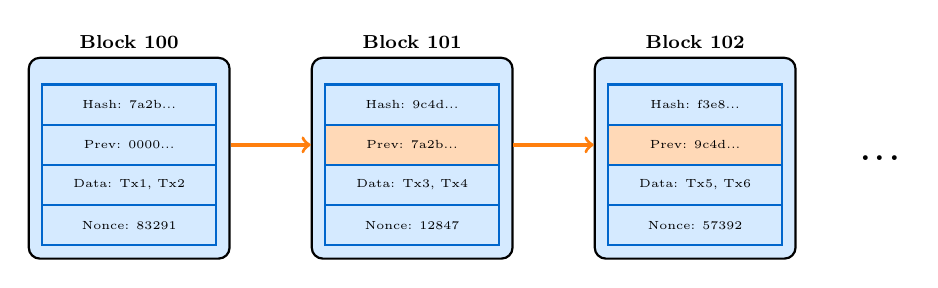
\begin{tikzpicture}[node distance=0.3cm, scale=0.85, transform shape]
% Block 1
\node[draw, thick, rounded corners, minimum width=3cm, minimum height=3cm, fill=dflightblue4] (b1) {};
\node[above=0mm of b1.north, font=\bfseries\footnotesize] {Block 100};
\node[databox, minimum width=2.6cm, font=\tiny] at ($(b1.center) + (0,0.8)$) {Hash: 7a2b...};
\node[databox, minimum width=2.6cm, font=\tiny] at ($(b1.center) + (0,0.2)$) {Prev: 0000...};
\node[databox, minimum width=2.6cm, font=\tiny] at ($(b1.center) + (0,-0.4)$) {Data: Tx1, Tx2};
\node[databox, minimum width=2.6cm, font=\tiny] at ($(b1.center) + (0,-1)$) {Nonce: 83291};

% Block 2
\node[draw, thick, rounded corners, minimum width=3cm, minimum height=3cm, fill=dflightblue4, right=1.2cm of b1] (b2) {};
\node[above=0mm of b2.north, font=\bfseries\footnotesize] {Block 101};
\node[databox, minimum width=2.6cm, font=\tiny] at ($(b2.center) + (0,0.8)$) {Hash: 9c4d...};
\node[databox, minimum width=2.6cm, font=\tiny, fill=dforange!30] at ($(b2.center) + (0,0.2)$) {Prev: 7a2b...};
\node[databox, minimum width=2.6cm, font=\tiny] at ($(b2.center) + (0,-0.4)$) {Data: Tx3, Tx4};
\node[databox, minimum width=2.6cm, font=\tiny] at ($(b2.center) + (0,-1)$) {Nonce: 12847};

% Block 3
\node[draw, thick, rounded corners, minimum width=3cm, minimum height=3cm, fill=dflightblue4, right=1.2cm of b2] (b3) {};
\node[above=0mm of b3.north, font=\bfseries\footnotesize] {Block 102};
\node[databox, minimum width=2.6cm, font=\tiny] at ($(b3.center) + (0,0.8)$) {Hash: f3e8...};
\node[databox, minimum width=2.6cm, font=\tiny, fill=dforange!30] at ($(b3.center) + (0,0.2)$) {Prev: 9c4d...};
\node[databox, minimum width=2.6cm, font=\tiny] at ($(b3.center) + (0,-0.4)$) {Data: Tx5, Tx6};
\node[databox, minimum width=2.6cm, font=\tiny] at ($(b3.center) + (0,-1)$) {Nonce: 57392};

% Linking arrows
\draw[very thick, dforange, ->] ($(b1.east) + (0,0.2)$) -- ($(b2.west) + (0,0.2)$);
\draw[very thick, dforange, ->] ($(b2.east) + (0,0.2)$) -- ($(b3.west) + (0,0.2)$);

% Future blocks
\node[right=0.8cm of b3, font=\Huge] {...};
\end{tikzpicture}
\end{center}

\vspace{3mm}
\textbf{The chain property:} Each block contains the hash of the previous block

\textbf{Why this matters:} Change Block 100 $\rightarrow$ its hash changes $\rightarrow$ Block 101's ``Prev'' becomes invalid $\rightarrow$ cascading invalidity

\bottomnote{This is why blockchain history is considered immutable}
\end{frame}

\begin{frame}{Why Tampering Is Detectable}
\begin{center}
\begin{tabular}{c|c}
\textbf{Original Chain} & \textbf{Tampered Chain} \\
\hline
& \\
Block 100: Hash = 7a2b... & Block 100: Hash = \textcolor{dfred}{x9f2...} \\
$\downarrow$ (valid link) & $\downarrow$ \textcolor{dfred}{(broken link!)} \\
Block 101: Prev = 7a2b... & Block 101: Prev = 7a2b... \textcolor{dfred}{X} \\
$\downarrow$ (valid link) & $\downarrow$ \textcolor{dfred}{(broken link!)} \\
Block 102: Prev = 9c4d... & Block 102: Prev = 9c4d... \textcolor{dfred}{X} \\
& \\
\textcolor{dfgreen}{\checkmark Valid} & \textcolor{dfred}{X Invalid} \\
\end{tabular}
\end{center}

\vspace{5mm}
\textbf{To tamper with history, attacker must:}
\begin{enumerate}
\item Change the target block's data
\item Recalculate that block's hash
\item Recalculate \textit{every subsequent block's hash}
\item Do this faster than the honest network adds new blocks
\end{enumerate}

\textcolor{dfred}{Practically impossible once blocks are deep in the chain}
\end{frame}

\begin{frame}{The Consensus Problem}
\begin{columns}[T]
\begin{column}{0.55\textwidth}
\textbf{The Challenge}

In a decentralized network:
\begin{itemize}
\item No central authority
\item Nodes don't trust each other
\item Messages can be delayed or lost
\item Some nodes may be malicious
\end{itemize}

\vspace{3mm}
\textbf{The Question}

How do thousands of strangers agree on:
\begin{itemize}
\item Which transactions are valid?
\item What order do they go in?
\item What is the ``true'' history?
\end{itemize}
\end{column}
\begin{column}{0.42\textwidth}
\begin{center}
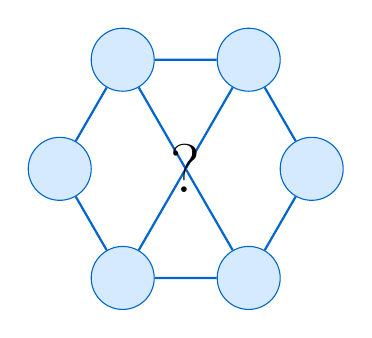
\begin{tikzpicture}[scale=0.8]
% Network of nodes
\foreach \i in {1,...,6} {
    \node[circle, draw=dfblue, fill=dflightblue4, minimum size=0.8cm] (n\i) at ({60*\i}:2) {};
}
% Some connections
\draw[thick, dfblue] (n1) -- (n2);
\draw[thick, dfblue] (n2) -- (n3);
\draw[thick, dfblue] (n3) -- (n4);
\draw[thick, dfblue] (n4) -- (n5);
\draw[thick, dfblue] (n5) -- (n6);
\draw[thick, dfblue] (n6) -- (n1);
\draw[thick, dfblue] (n1) -- (n4);
\draw[thick, dfblue] (n2) -- (n5);

% Question mark in center
\node[font=\Huge] at (0,0) {?};
\end{tikzpicture}

\footnotesize Who decides the truth?
\end{center}
\end{column}
\end{columns}

\vspace{3mm}
\begin{block}{Consensus Mechanism}
A set of rules that allows a distributed network to agree on a single version of truth, even in the presence of faulty or malicious participants.
\end{block}
\end{frame}

\begin{frame}{Proof of Work (PoW): Bitcoin's Answer}
\begin{center}
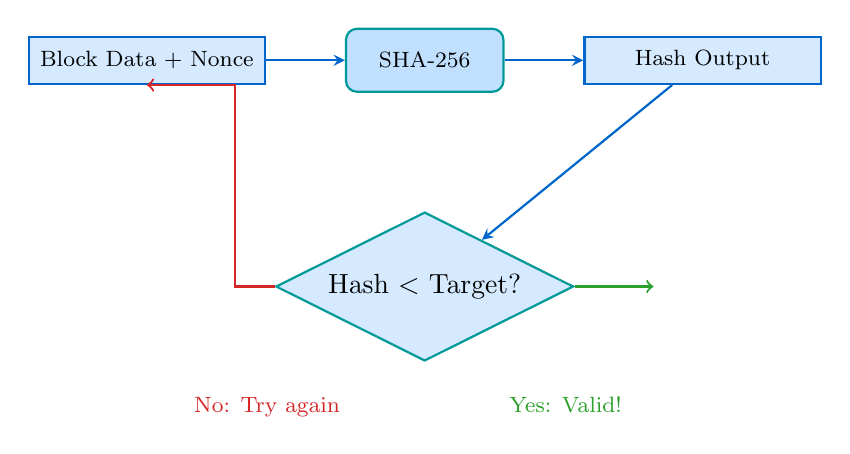
\begin{tikzpicture}[node distance=0.5cm]
% Mining process
\node[databox, minimum width=3cm] (block) {Block Data + Nonce};
\node[hashbox, right=1cm of block, minimum width=2cm] (hash) {SHA-256};
\node[databox, right=1cm of hash, minimum width=3cm] (output) {Hash Output};

\draw[arrow] (block) -- (hash);
\draw[arrow] (hash) -- (output);

% Condition
\node[decision, below=1.5cm of hash, minimum width=2.5cm, aspect=2] (check) {Hash $<$ Target?};

% Outcomes
\node[below left=0.8cm and 0cm of check, font=\footnotesize, text=dfred] (no) {No: Try again};
\node[below right=0.8cm and 0cm of check, font=\footnotesize, text=dfgreen] (yes) {Yes: Valid!};

\draw[arrow] (output) -- (check);
\draw[thick, dfred, ->] (check.west) -- ++(-0.5,0) |- (block.south);
\draw[thick, dfgreen, ->] (check.east) -- ++(1,0);
\end{tikzpicture}
\end{center}

\vspace{3mm}
\textbf{The ``work'' in Proof of Work:}
\begin{itemize}
\item Find a nonce that makes the block hash start with many zeros
\item Requires billions of guesses (brute force)
\item Easy to verify: just hash once and check
\item Hard to produce: requires massive computation
\end{itemize}
\end{frame}

\begin{frame}{Proof of Work: Security Through Energy}
\begin{columns}[T]
\begin{column}{0.48\textwidth}
\textbf{Why It Works}
\begin{itemize}\compactlist
\item Attack requires controlling 51\% of computing power
\item This costs billions in hardware + electricity
\item Rational: mining honestly is more profitable
\item Economic security: attack cost $>$ potential gain
\end{itemize}

\vspace{3mm}
\textbf{Advantages}
\begin{itemize}\compactlist
\item Battle-tested (Bitcoin since 2009)
\item Highly secure
\item Truly decentralized
\end{itemize}
\end{column}
\begin{column}{0.48\textwidth}
\textbf{Criticisms}
\begin{itemize}\compactlist
\item \textcolor{dfred}{Enormous energy consumption}
\item Bitcoin uses more electricity than some countries
\item Environmental concerns
\item Hardware arms race (specialized ASICs)
\end{itemize}

\vspace{3mm}
\begin{center}
\fbox{\parbox{0.8\textwidth}{\centering
Bitcoin Network:\\
$\approx$ 150 TWh/year\\
{\footnotesize (more than Argentina)}
}}
\end{center}
\end{column}
\end{columns}

\bottomnote{PoW trades energy for security -- the ``work'' is the cost of attack}
\end{frame}

\begin{frame}{Proof of Stake (PoS): Ethereum's Answer}
\begin{center}
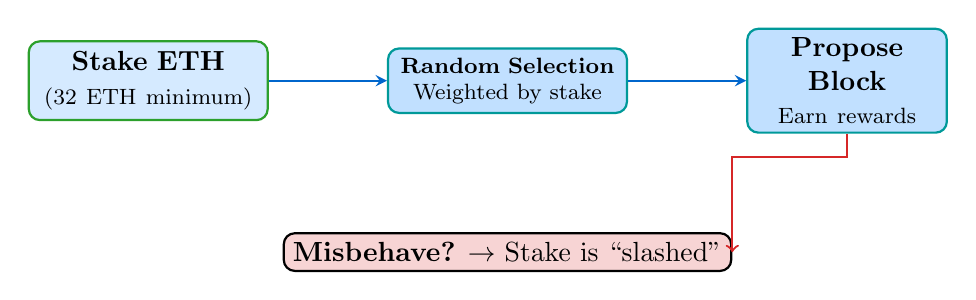
\begin{tikzpicture}[node distance=0.8cm]
% Staking process
\node[walletbox, minimum width=3cm, text width=2.8cm, align=center] (stake) {
\textbf{Stake ETH}\\
\footnotesize (32 ETH minimum)
};

\node[hashbox, right=1.5cm of stake, minimum width=3cm, text width=2.8cm, align=center] (select) {
\textbf{Random Selection}\\
\footnotesize Weighted by stake
};

\node[blocknode, right=1.5cm of select, minimum width=2.5cm, minimum height=1.2cm, text width=2.3cm, align=center] (propose) {
\textbf{Propose Block}\\
\footnotesize Earn rewards
};

\draw[arrow] (stake) -- (select);
\draw[arrow] (select) -- (propose);

% Slashing
\node[below=1.5cm of select, draw, thick, rounded corners, fill=dfred!20, minimum width=5cm] (slash) {
\textbf{Misbehave?} $\rightarrow$ Stake is ``slashed''
};
\draw[thick, dfred, ->] (propose.south) -- ++(0,-0.3) -| (slash.east);
\end{tikzpicture}
\end{center}

\vspace{3mm}
\textbf{The ``stake'' in Proof of Stake:}
\begin{itemize}
\item Lock up cryptocurrency as collateral
\item More stake = higher chance to be selected as validator
\item Honest behavior = earn rewards
\item Malicious behavior = lose your stake (``slashing'')
\end{itemize}
\end{frame}

\begin{frame}{PoW vs. PoS: Head-to-Head Comparison}
\begin{center}
\begin{tabular}{l|c|c}
\toprule
\textbf{Aspect} & \textbf{Proof of Work} & \textbf{Proof of Stake} \\
\midrule
Security basis & Computational power & Economic stake \\
Energy usage & \textcolor{dfred}{Very high} & \textcolor{dfgreen}{Low ($\sim$99.9\% less)} \\
Hardware required & Specialized (ASICs) & Standard computers \\
Entry barrier & High (equipment cost) & High (32 ETH) \\
Attack cost & Hardware + electricity & Acquire 51\% of stake \\
Decentralization & Mining pool concentration & Wealth concentration \\
Finality & Probabilistic & Faster, more definite \\
Examples & Bitcoin, Dogecoin & Ethereum, Cardano, Solana \\
\bottomrule
\end{tabular}
\end{center}

\vspace{3mm}
\textbf{Key insight:} Neither is ``better'' -- they make different tradeoffs

\bottomnote{Ethereum transitioned from PoW to PoS in Sept 2022 (``The Merge'')}
\end{frame}

\begin{frame}{The Blockchain Trilemma}
\begin{center}
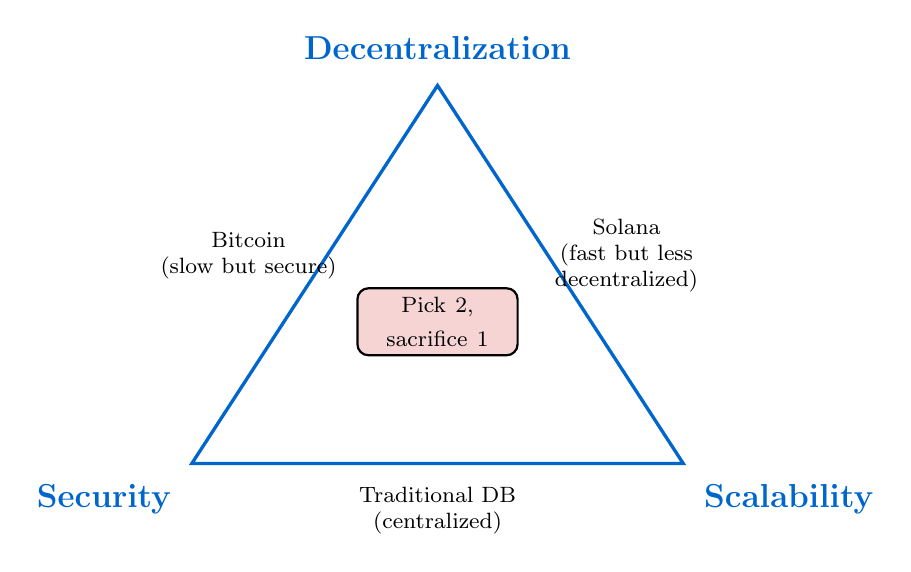
\begin{tikzpicture}[scale=1.2]
% Triangle
\coordinate (D) at (0, 3);
\coordinate (Se) at (-2.6, -1);
\coordinate (Sc) at (2.6, -1);

\draw[very thick, dfblue] (D) -- (Se) -- (Sc) -- cycle;

% Labels
\node[above=2mm of D, font=\bfseries\large, text=dfblue] {Decentralization};
\node[below left=2mm of Se, font=\bfseries\large, text=dfblue] {Security};
\node[below right=2mm of Sc, font=\bfseries\large, text=dfblue] {Scalability};

% Center impossible zone
\node[draw, thick, rounded corners, fill=dfred!20, minimum width=2cm, text width=1.8cm, align=center] at (0, 0.5) {
\footnotesize Pick 2,\\
sacrifice 1
};

% Examples on edges
\node[font=\footnotesize, text width=2.3cm, align=center] at (-2, 1.2) {Bitcoin\\(slow but secure)};
\node[font=\footnotesize, text width=2.3cm, align=center] at (2, 1.2) {Solana\\(fast but less\\decentralized)};
\node[font=\footnotesize, text width=2.3cm, align=center] at (0, -1.5) {Traditional DB\\(centralized)};
\end{tikzpicture}
\end{center}
\end{frame}

\begin{frame}{The Trilemma Explained}
\begin{columns}[T]
\begin{column}{0.32\textwidth}
\textbf{Decentralization}
\begin{itemize}\compactlist
\item Many independent validators
\item No single point of control
\item Censorship resistant
\item Geographic distribution
\end{itemize}
\textcolor{dfred}{Tradeoff: More nodes = slower}
\end{column}
\begin{column}{0.32\textwidth}
\textbf{Security}
\begin{itemize}\compactlist
\item Resistant to attacks
\item Immutable history
\item Byzantine fault tolerant
\item Economic finality
\end{itemize}
\textcolor{dfred}{Tradeoff: More verification = slower}
\end{column}
\begin{column}{0.32\textwidth}
\textbf{Scalability}
\begin{itemize}\compactlist
\item High throughput (TPS)
\item Low latency
\item Low fees
\item Handle demand spikes
\end{itemize}
\textcolor{dfred}{Tradeoff: Speed often requires centralization}
\end{column}
\end{columns}

\vspace{5mm}
\begin{center}
\begin{tabular}{l|ccc}
\toprule
\textbf{System} & \textbf{TPS} & \textbf{Finality} & \textbf{Validators} \\
\midrule
Bitcoin & 7 & 60 min & $\sim$15,000 nodes \\
Ethereum & 15-30 & 12-15 min & $\sim$500,000 validators \\
Solana & 65,000 & 0.4 sec & $\sim$1,900 validators \\
Visa & 24,000 & seconds & 1 (centralized) \\
\bottomrule
\end{tabular}
\end{center}
\end{frame}

\begin{frame}{Scaling Solutions: Breaking the Trilemma?}
\begin{columns}[T]
\begin{column}{0.48\textwidth}
\textbf{Layer 1 Solutions}

\textit{Improve the base blockchain}
\begin{itemize}\compactlist
\item Larger blocks (more data per block)
\item Faster block times
\item More efficient consensus
\item Sharding (parallel processing)
\end{itemize}

\vspace{3mm}
\textbf{Examples:}
\begin{itemize}\compactlist
\item Ethereum 2.0 (sharding planned)
\item Solana (parallel processing)
\item Near Protocol (sharding)
\end{itemize}
\end{column}
\begin{column}{0.48\textwidth}
\textbf{Layer 2 Solutions}

\textit{Build on top of base layer}
\begin{itemize}\compactlist
\item Process transactions off-chain
\item Settle on main chain periodically
\item Inherit security from L1
\item Much higher throughput
\end{itemize}

\vspace{3mm}
\textbf{Examples:}
\begin{itemize}\compactlist
\item Lightning Network (Bitcoin)
\item Optimism, Arbitrum (Ethereum)
\item Polygon (Ethereum)
\end{itemize}
\end{column}
\end{columns}

\vspace{3mm}
\begin{block}{Key Insight}
Layer 2 solutions let blockchains scale WITHOUT sacrificing decentralization or security at the base layer.
\end{block}
\end{frame}

\begin{frame}{Summary: How Blockchains Work}
\begin{center}
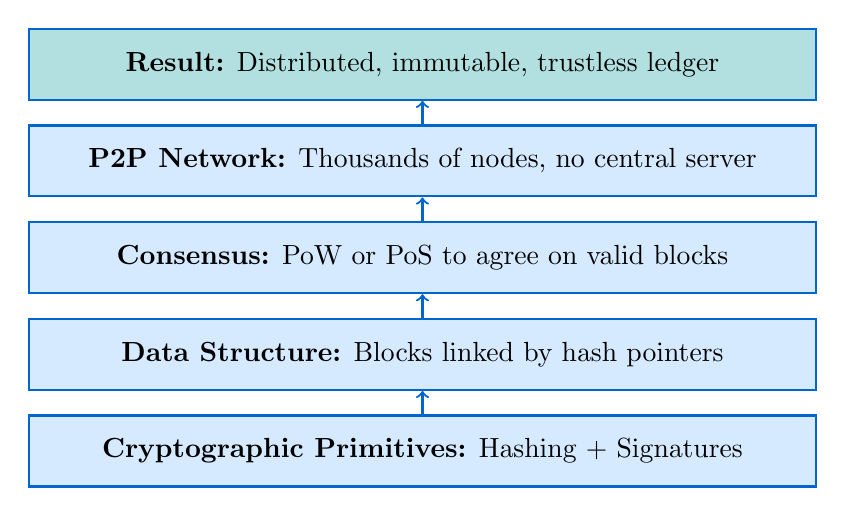
\begin{tikzpicture}[node distance=0.3cm]
% Layers
\node[process, minimum width=10cm, minimum height=0.9cm] (l1) {
\textbf{Cryptographic Primitives:} Hashing + Signatures
};
\node[process, minimum width=10cm, minimum height=0.9cm, above=of l1] (l2) {
\textbf{Data Structure:} Blocks linked by hash pointers
};
\node[process, minimum width=10cm, minimum height=0.9cm, above=of l2] (l3) {
\textbf{Consensus:} PoW or PoS to agree on valid blocks
};
\node[process, minimum width=10cm, minimum height=0.9cm, above=of l3] (l4) {
\textbf{P2P Network:} Thousands of nodes, no central server
};
\node[process, minimum width=10cm, minimum height=0.9cm, fill=dfteal!30, above=of l4] (l5) {
\textbf{Result:} Distributed, immutable, trustless ledger
};

\draw[thick, dfblue, ->] (l1.north) -- (l2.south);
\draw[thick, dfblue, ->] (l2.north) -- (l3.south);
\draw[thick, dfblue, ->] (l3.north) -- (l4.south);
\draw[thick, dfblue, ->] (l4.north) -- (l5.south);
\end{tikzpicture}
\end{center}

\vspace{3mm}
\textbf{The fundamental tradeoff:} Blockchains sacrifice efficiency for trust minimization. When you need trustless coordination among strangers, this tradeoff is worth it.

\bottomnote{Hands-on: NB06 -- Build a mini-blockchain and simulate tampering}
\end{frame}

% =======================================================================
% SECTION 3.3: WALLETS, TRANSACTIONS & UX GAP
% =======================================================================
\section{3.3 Wallets, Transactions \& UX Gap}

\begin{frame}{From Theory to Practice: How Users Interact}
\begin{center}
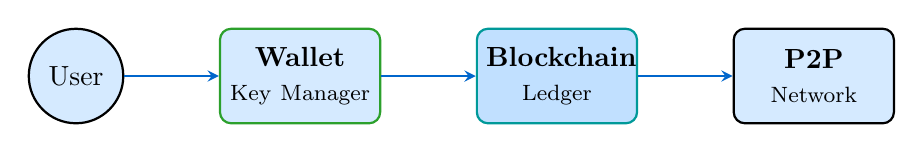
\begin{tikzpicture}[node distance=1cm]
% User
\node[draw, thick, circle, minimum size=1.2cm, fill=dflightblue4] (user) {User};

% Wallet
\node[walletbox, right=1.2cm of user, minimum width=2cm, minimum height=1.2cm, text width=1.8cm, align=center] (wallet) {
\textbf{Wallet}\\
\footnotesize Key Manager
};

% Blockchain
\node[blocknode, right=1.2cm of wallet, minimum width=2cm, minimum height=1.2cm, text width=1.8cm, align=center] (bc) {
\textbf{Blockchain}\\
\footnotesize Ledger
};

% Network
\node[draw, thick, rounded corners, minimum width=2cm, minimum height=1.2cm, fill=dflightblue4, right=1.2cm of bc, text width=1.8cm, align=center] (network) {
\textbf{P2P}\\
\footnotesize Network
};

\draw[arrow] (user) -- (wallet);
\draw[arrow] (wallet) -- (bc);
\draw[arrow] (bc) -- (network);
\end{tikzpicture}
\end{center}

\vspace{5mm}
\textbf{Key insight:} Users never interact with the blockchain directly.

The \textbf{wallet} is the interface -- it manages keys, signs transactions, and broadcasts them to the network.

\begin{block}{Common Misconception}
Wallets don't ``store'' cryptocurrency. The blockchain stores balances.\\
Wallets store \textit{keys} that prove you can spend those balances.
\end{block}
\end{frame}

\begin{frame}{What Is a Wallet, Really?}
\begin{columns}[T]
\begin{column}{0.55\textwidth}
\textbf{A wallet is a key management tool}

It does three things:
\begin{enumerate}
\item \textbf{Stores private keys} (securely, hopefully)
\item \textbf{Signs transactions} using those keys
\item \textbf{Broadcasts transactions} to the network
\end{enumerate}

\vspace{3mm}
\textbf{It does NOT:}
\begin{itemize}
\item Store cryptocurrency
\item Connect you to a bank
\item Know your identity
\item Require permission to create
\end{itemize}
\end{column}
\begin{column}{0.42\textwidth}
\begin{center}
\fbox{\parbox{0.9\textwidth}{
\textbf{Wallet Contents}\\[3mm]
\textcolor{dfred}{Private Key 1}\\
{\tiny 0x7a2b...secret}\\[2mm]
\textcolor{dfgreen}{Address 1: 0x9c4d...}\\[1mm]
\textcolor{dfgreen}{Address 2: 0xf3e8...}\\[2mm]
Balance: 1.5 ETH\\
{\tiny (queried from blockchain)}
}}
\end{center}
\end{column}
\end{columns}
\end{frame}

\begin{frame}{Types of Wallets: A Spectrum of Tradeoffs}
\begin{center}
\textbf{Security vs. Convenience Tradeoff}

\vspace{3mm}
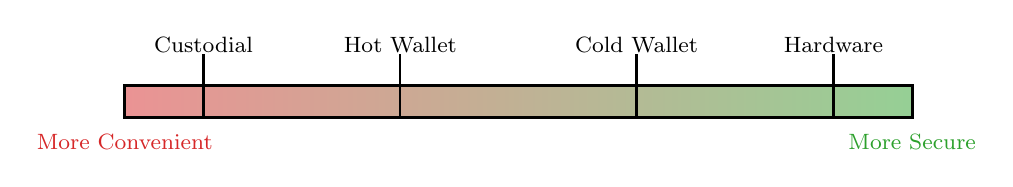
\begin{tikzpicture}
% Spectrum bar
\draw[very thick, left color=dfred!50, right color=dfgreen!50] (-5,-0.2) rectangle (5,0.2);
\node[below=0.3cm, font=\footnotesize] at (-5,0) {\textcolor{dfred}{More Convenient}};
\node[below=0.3cm, font=\footnotesize] at (5,0) {\textcolor{dfgreen}{More Secure}};

% Wallet types
\node[above=0.5cm] at (-4, 0) {\footnotesize Custodial};
\node[above=0.5cm] at (-1.5, 0) {\footnotesize Hot Wallet};
\node[above=0.5cm] at (1.5, 0) {\footnotesize Cold Wallet};
\node[above=0.5cm] at (4, 0) {\footnotesize Hardware};

\draw[thick] (-4, -0.2) -- (-4, 0.6);
\draw[thick] (-1.5, -0.2) -- (-1.5, 0.6);
\draw[thick] (1.5, -0.2) -- (1.5, 0.6);
\draw[thick] (4, -0.2) -- (4, 0.6);
\end{tikzpicture}
\end{center}

\vspace{5mm}
\begin{tabular}{l|l|l|l}
\toprule
\textbf{Type} & \textbf{Key Control} & \textbf{Example} & \textbf{Risk} \\
\midrule
Custodial & Exchange holds keys & Coinbase, Binance & Exchange hack \\
Hot Wallet & You hold, online & MetaMask & Malware, phishing \\
Cold Wallet & You hold, offline & Paper wallet & Physical loss \\
Hardware & You hold, secure chip & Ledger, Trezor & Device failure \\
\bottomrule
\end{tabular}
\end{frame}

\begin{frame}{Custodial vs. Non-Custodial: Who Holds the Keys?}
\begin{columns}[T]
\begin{column}{0.48\textwidth}
\textbf{Custodial (Exchange) Wallet}

You $\rightarrow$ Exchange $\rightarrow$ Blockchain

\vspace{3mm}
\begin{itemize}\compactlist
\item \textcolor{dfgreen}{Easy to use}
\item \textcolor{dfgreen}{Password recovery possible}
\item \textcolor{dfgreen}{Fiat on/off ramps}
\item \textcolor{dfred}{You don't control keys}
\item \textcolor{dfred}{Exchange can freeze funds}
\item \textcolor{dfred}{Exchange can be hacked}
\end{itemize}
\end{column}
\begin{column}{0.48\textwidth}
\textbf{Non-Custodial (Self-Custody)}

You $\rightarrow$ Your Wallet $\rightarrow$ Blockchain

\vspace{3mm}
\begin{itemize}\compactlist
\item \textcolor{dfgreen}{Full control}
\item \textcolor{dfgreen}{No counterparty risk}
\item \textcolor{dfgreen}{Censorship resistant}
\item \textcolor{dfred}{You are responsible}
\item \textcolor{dfred}{Lose keys = lose funds}
\item \textcolor{dfred}{No customer support}
\end{itemize}
\end{column}
\end{columns}

\vspace{5mm}
\begin{center}
\fbox{\parbox{0.6\textwidth}{\centering
\textbf{``Not your keys, not your coins''}\\
\footnotesize FTX collapse (2022): \$8B in customer funds lost
}}
\end{center}
\end{frame}

\begin{frame}{Anatomy of a Blockchain Transaction}
\begin{center}
\textbf{Ethereum Transaction Structure}

\vspace{3mm}
\begin{tabular}{|l|l|l|}
\hline
\textbf{Field} & \textbf{Value} & \textbf{Purpose} \\
\hline
From & 0x7a2b...9f3c & Sender's address \\
To & 0x9c4d...e8f2 & Recipient's address \\
Value & 1.5 ETH & Amount to transfer \\
Nonce & 42 & Tx count (prevents replay) \\
Gas Limit & 21,000 & Max computation units \\
Gas Price & 50 gwei & Price per gas unit \\
\hline
\textbf{Signature} & v, r, s & Proves authorization \\
\hline
\end{tabular}
\end{center}

\vspace{5mm}
The signature covers ALL fields above it -- proving the sender authorized this exact transaction.
\end{frame}

\begin{frame}{Understanding Gas: The Cost of Computation}
\begin{columns}[T]
\begin{column}{0.55\textwidth}
\textbf{What is Gas?}
\begin{itemize}\compactlist
\item Unit measuring computational work
\item Each operation has a gas cost
\item Simple transfer: 21,000 gas
\item Smart contract call: varies (100K+)
\end{itemize}

\vspace{3mm}
\textbf{Gas Economics}

\[
\text{Fee} = \text{Gas Used} \times \text{Gas Price}
\]

\vspace{2mm}
\textbf{Example:}
\begin{itemize}\compactlist
\item Gas used: 21,000
\item Gas price: 50 gwei
\item Fee = 21,000 $\times$ 50 gwei = 0.00105 ETH
\end{itemize}
\end{column}
\begin{column}{0.42\textwidth}
\textbf{Why Gas Exists}
\begin{enumerate}\compactlist
\item Prevents infinite loops
\item Compensates validators
\item Prioritizes transactions
\item Allocates scarce block space
\end{enumerate}

\vspace{3mm}
\begin{center}
\fbox{\parbox{0.9\textwidth}{
\textbf{Network Congestion}\\[2mm]
High demand $\rightarrow$\\
Higher gas prices $\rightarrow$\\
Higher fees\\[2mm]
\footnotesize (Supply and demand)
}}
\end{center}
\end{column}
\end{columns}

\bottomnote{Gas prices fluctuate wildly -- from cents to hundreds of dollars per transaction}
\end{frame}

\begin{frame}{The User Experience Gap}
\begin{center}
\textbf{What crypto asks users to understand:}
\end{center}

\begin{columns}[T]
\begin{column}{0.48\textwidth}
\begin{center}
\textbf{Traditional Banking}
\end{center}
\begin{itemize}\compactlist
\item Username and password
\item ``Forgot password?'' link
\item Customer support
\item FDIC insurance
\item Fraud protection
\item Clear error messages
\end{itemize}

\vspace{3mm}
\begin{center}
\textcolor{dfgreen}{Forgiving of mistakes}
\end{center}
\end{column}
\begin{column}{0.48\textwidth}
\begin{center}
\textbf{Cryptocurrency}
\end{center}
\begin{itemize}\compactlist
\item 24-word seed phrase
\item Lose phrase = lose everything
\item No customer support
\item No insurance (usually)
\item Irreversible transactions
\item Cryptic error: ``insufficient gas''
\end{itemize}

\vspace{3mm}
\begin{center}
\textcolor{dfred}{Unforgiving of mistakes}
\end{center}
\end{column}
\end{columns}

\vspace{3mm}
\begin{block}{The UX Problem}
Crypto's security model requires users to be their own bank.\\
Most people don't want that responsibility.
\end{block}
\end{frame}

\begin{frame}{Common User Errors (And Their Consequences)}
\begin{center}
\begin{tabular}{l|l|l}
\toprule
\textbf{Error} & \textbf{Consequence} & \textbf{Recovery?} \\
\midrule
Lost seed phrase & Permanent loss of funds & \textcolor{dfred}{No} \\
Sent to wrong address & Funds gone forever & \textcolor{dfred}{No} \\
Wrong network (ETH to BSC) & Funds stuck/lost & \textcolor{dforange}{Sometimes} \\
Insufficient gas & Transaction fails & \textcolor{dfgreen}{Yes, retry} \\
Approved malicious contract & Wallet drained & \textcolor{dfred}{No} \\
Phishing attack & Keys stolen & \textcolor{dfred}{No} \\
Didn't verify contract & Funds stolen & \textcolor{dfred}{No} \\
\bottomrule
\end{tabular}
\end{center}

\vspace{5mm}
\textbf{Scale of the problem:}
\begin{itemize}
\item \$3.8 billion lost to crypto hacks in 2022 (Chainalysis)
\item Estimated 20\% of Bitcoin permanently inaccessible (lost keys)
\item Phishing remains the \#1 attack vector
\end{itemize}
\end{frame}

\begin{frame}{Improving Crypto UX: Current Efforts}
\begin{columns}[T]
\begin{column}{0.48\textwidth}
\textbf{Technical Solutions}
\begin{itemize}\compactlist
\item \textbf{Account abstraction:} Smart contract wallets with recovery
\item \textbf{Social recovery:} Trusted friends can help recover
\item \textbf{Multi-sig:} Require multiple keys to transact
\item \textbf{Hardware wallets:} Secure key storage
\item \textbf{ENS names:} Human-readable addresses
\end{itemize}
\end{column}
\begin{column}{0.48\textwidth}
\textbf{UX Improvements}
\begin{itemize}\compactlist
\item \textbf{Transaction simulation:} Show what will happen before signing
\item \textbf{Clear warnings:} ``This will drain your wallet''
\item \textbf{Gas estimation:} Show fees in dollars
\item \textbf{Address books:} Saved, verified addresses
\item \textbf{Better error messages:} Human-readable explanations
\end{itemize}
\end{column}
\end{columns}

\vspace{5mm}
\begin{block}{The Goal}
Make self-custody as easy as using a bank app, without sacrificing security or decentralization.
\end{block}

\bottomnote{Hands-on: NB07 -- Construct and examine transactions on a testnet}
\end{frame}

\begin{frame}{Summary: The Wallet Landscape}
\textbf{Decision tree for choosing a wallet:}

\vspace{3mm}
\begin{enumerate}
\item \textbf{Who holds the keys?}
\begin{itemize}
\item Exchange holds them $\rightarrow$ \textbf{Custodial} (easy, but risky)
\item You hold them $\rightarrow$ Continue to step 2
\end{itemize}

\vspace{2mm}
\item \textbf{Is it connected to the internet?}
\begin{itemize}
\item Yes $\rightarrow$ \textbf{Hot wallet} (MetaMask) -- convenient for daily use
\item No $\rightarrow$ \textbf{Cold/Hardware wallet} (Ledger) -- secure for savings
\end{itemize}
\end{enumerate}

\vspace{5mm}
\textbf{Key Takeaway:} Wallet choice = tradeoff between convenience and security.\\
Most users need \textit{both}: hot wallet for daily use, cold storage for savings.
\end{frame}

% =======================================================================
% SECTION 3.4: BITCOIN VS. ETHEREUM
% =======================================================================
\section{3.4 Bitcoin vs. Ethereum}

\begin{frame}{Two Visions of Blockchain}
\begin{columns}[T]
\begin{column}{0.48\textwidth}
\begin{center}
\textbf{\Large Bitcoin}\\[2mm]
\textit{``Digital Gold''}
\end{center}

\vspace{3mm}
\begin{itemize}\compactlist
\item Store of value
\item Fixed supply (21M)
\item Minimal, robust
\item Conservative changes
\item ``Don't break what works''
\end{itemize}

\vspace{3mm}
\begin{center}
\fbox{\parbox{0.85\textwidth}{\centering
\textbf{Goal:} Sound money that\\no one can inflate or censor
}}
\end{center}
\end{column}
\begin{column}{0.48\textwidth}
\begin{center}
\textbf{\Large Ethereum}\\[2mm]
\textit{``World Computer''}
\end{center}

\vspace{3mm}
\begin{itemize}\compactlist
\item Platform for applications
\item Programmable money
\item Feature-rich, flexible
\item Active development
\item ``Move fast, iterate''
\end{itemize}

\vspace{3mm}
\begin{center}
\fbox{\parbox{0.85\textwidth}{\centering
\textbf{Goal:} Decentralized platform\\for any application
}}
\end{center}
\end{column}
\end{columns}
\end{frame}

\begin{frame}{Historical Context}
\begin{center}
\begin{tabular}{c|l}
\textbf{Year} & \textbf{Event} \\
\hline
2009 & Bitcoin launches \\
2012 & Colored coins on Bitcoin (limited tokens) \\
2013 & Ethereum whitepaper (Vitalik Buterin) \\
2015 & Ethereum launches \\
2022 & Ethereum transitions to Proof of Stake \\
\end{tabular}
\end{center}

\vspace{5mm}
\textbf{Vitalik Buterin's insight (2013):}

Bitcoin's scripting language was too limited. He proposed a blockchain with a \textbf{Turing-complete} programming language -- one that could run any program, not just simple transactions.

\begin{block}{The Key Difference}
Bitcoin: ``Is this a valid payment?'' (simple yes/no)\\
Ethereum: ``Run this arbitrary code and tell me the result'' (general computation)
\end{block}
\end{frame}

\begin{frame}{Technical Comparison: Head to Head}
\begin{center}
\begin{tabular}{l|c|c}
\toprule
\textbf{Feature} & \textbf{Bitcoin} & \textbf{Ethereum} \\
\midrule
Launch & 2009 & 2015 \\
Consensus & Proof of Work & Proof of Stake (since 2022) \\
Block time & $\sim$10 minutes & $\sim$12 seconds \\
Supply cap & 21 million BTC & No hard cap \\
Issuance & Halving every 4 years & Dynamic (can be deflationary) \\
Scripting & Limited (Bitcoin Script) & Turing-complete (EVM) \\
Primary use & Value transfer, store of value & Smart contracts, DeFi, NFTs \\
TPS & $\sim$7 & $\sim$15-30 \\
\bottomrule
\end{tabular}
\end{center}

\vspace{3mm}
\textbf{Key insight:} These aren't competing for the same use case.\\
Bitcoin optimizes for \textit{security and immutability}.\\
Ethereum optimizes for \textit{programmability and flexibility}.
\end{frame}

\begin{frame}{Bitcoin: The Sound Money Thesis}
\begin{columns}[T]
\begin{column}{0.55\textwidth}
\textbf{Core Properties}
\begin{itemize}\compactlist
\item \textbf{Fixed supply:} 21 million, ever
\item \textbf{Predictable issuance:} Halving every 210,000 blocks
\item \textbf{Decentralized:} No one controls it
\item \textbf{Censorship resistant:} Anyone can transact
\item \textbf{Immutable:} Rules don't change
\end{itemize}

\vspace{3mm}
\textbf{The Narrative}
\begin{itemize}\compactlist
\item ``Digital gold'' -- scarce, durable
\item Hedge against inflation
\item Separation of money and state
\item Base layer for financial system
\end{itemize}
\end{column}
\begin{column}{0.42\textwidth}
\begin{center}
\textbf{Bitcoin Supply Curve}

\vspace{2mm}
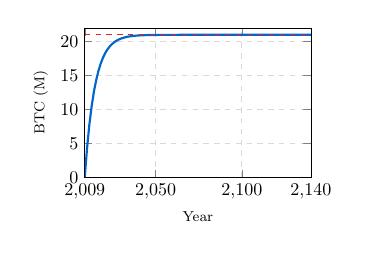
\begin{tikzpicture}[scale=0.65]
\begin{axis}[
    width=6cm, height=4.5cm,
    xlabel={\footnotesize Year},
    ylabel={\footnotesize BTC (M)},
    xmin=2009, xmax=2140,
    ymin=0, ymax=22,
    grid=major,
    grid style={dashed, gray!30},
    xtick={2009, 2050, 2100, 2140},
]
\addplot[very thick, dfblue, domain=2009:2140, samples=100]
    {21 * (1 - 2^(-(x-2009)/4))};
\addplot[dashed, dfred] coordinates {(2009,21) (2140,21)};
\end{axis}
\end{tikzpicture}

\footnotesize Asymptotically approaches 21M
\end{center}
\end{column}
\end{columns}

\bottomnote{Bitcoin maximalists: ``We already have one neutral, global money. Why do we need more?''}
\end{frame}

\begin{frame}{Ethereum: The World Computer Thesis}
\begin{columns}[T]
\begin{column}{0.55\textwidth}
\textbf{Core Properties}
\begin{itemize}\compactlist
\item \textbf{Smart contracts:} Self-executing code
\item \textbf{EVM:} Ethereum Virtual Machine
\item \textbf{Programmable:} Any logic possible
\item \textbf{Composable:} Contracts call contracts
\item \textbf{Tokens:} Create new assets easily
\end{itemize}

\vspace{3mm}
\textbf{The Narrative}
\begin{itemize}\compactlist
\item Platform for decentralized apps
\item ``DeFi'' -- finance without banks
\item NFTs, DAOs, and more
\item Base layer for Web3
\end{itemize}
\end{column}
\begin{column}{0.42\textwidth}
\begin{center}
\textbf{Ethereum Stack}

\vspace{2mm}
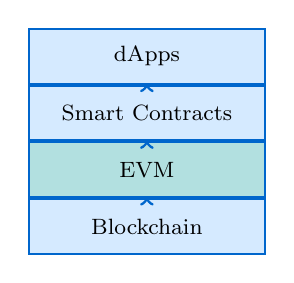
\begin{tikzpicture}[scale=0.8]
% EVM stack
\node[process, minimum width=3cm, minimum height=0.7cm] (l1) at (0,0) {\footnotesize dApps};
\node[process, minimum width=3cm, minimum height=0.7cm] (l2) at (0,-0.9) {\footnotesize Smart Contracts};
\node[process, minimum width=3cm, minimum height=0.7cm, fill=dfteal!30] (l3) at (0,-1.8) {\footnotesize EVM};
\node[process, minimum width=3cm, minimum height=0.7cm] (l4) at (0,-2.7) {\footnotesize Blockchain};

\draw[thick, dfblue, <->] (l1.south) -- (l2.north);
\draw[thick, dfblue, <->] (l2.south) -- (l3.north);
\draw[thick, dfblue, <->] (l3.south) -- (l4.north);
\end{tikzpicture}

\footnotesize Apps built on contracts on EVM
\end{center}
\end{column}
\end{columns}

\bottomnote{Ethereum enables ``programmable money'' -- money with built-in rules}
\end{frame}

\begin{frame}{What Are Smart Contracts?}
\begin{columns}[T]
\begin{column}{0.48\textwidth}
\textbf{Traditional Contract}

\begin{enumerate}\compactlist
\item Legal document
\item Human interpretation
\item Court enforcement
\item (Maybe) execution
\end{enumerate}

\vspace{3mm}
Requires: lawyers, courts, trust
\end{column}
\begin{column}{0.48\textwidth}
\textbf{Smart Contract}

\begin{enumerate}\compactlist
\item Code on blockchain
\item Automatic execution
\item No intermediaries
\item Guaranteed outcome
\end{enumerate}

\vspace{3mm}
Requires: only the code
\end{column}
\end{columns}

\vspace{5mm}
\begin{block}{Definition}
A smart contract is code stored on a blockchain that automatically executes when predetermined conditions are met.

\textbf{Key property:} Once deployed, the code cannot be changed. ``Code is law.''
\end{block}
\end{frame}

\begin{frame}{Smart Contract Example: Escrow}
\begin{columns}[T]
\begin{column}{0.48\textwidth}
\textbf{Traditional Escrow}
\begin{enumerate}\compactlist
\item Buyer sends money to escrow agent
\item Seller ships goods
\item Buyer confirms receipt
\item Escrow agent releases funds to seller
\end{enumerate}

\vspace{3mm}
\textbf{Problems:}
\begin{itemize}\compactlist
\item Trust the escrow agent
\item Agent takes a fee
\item Disputes are slow
\item Counterparty risk
\end{itemize}
\end{column}
\begin{column}{0.48\textwidth}
\textbf{Smart Contract Escrow}
\begin{enumerate}\compactlist
\item Buyer sends ETH to contract
\item Contract holds funds
\item Buyer calls \texttt{confirmReceipt()}
\item Contract automatically sends to seller
\end{enumerate}

\vspace{3mm}
\textbf{Advantages:}
\begin{itemize}\compactlist
\item Trust the code (auditable)
\item Minimal fees (just gas)
\item Instant execution
\item No counterparty risk
\end{itemize}
\end{column}
\end{columns}

\vspace{3mm}
\begin{center}
\fbox{\parbox{0.7\textwidth}{\centering
\textbf{Key insight:} Smart contracts replace trusted intermediaries with verified code.
}}
\end{center}
\end{frame}

\begin{frame}{What ``Programmable Money'' Enables}
\begin{columns}[T]
\begin{column}{0.32\textwidth}
\textbf{DeFi}
\begin{itemize}\compactlist
\item Lending/borrowing
\item Decentralized exchanges
\item Yield farming
\item Derivatives
\end{itemize}
\end{column}
\begin{column}{0.32\textwidth}
\textbf{NFTs/Tokens}
\begin{itemize}\compactlist
\item Digital ownership
\item Tokenized assets
\item Loyalty programs
\item Gaming items
\end{itemize}
\end{column}
\begin{column}{0.32\textwidth}
\textbf{DAOs}
\begin{itemize}\compactlist
\item Decentralized governance
\item Treasury management
\item Collective ownership
\item Voting systems
\end{itemize}
\end{column}
\end{columns}

\vspace{5mm}
\begin{center}
All built on Ethereum's programmable foundation
\end{center}

\vspace{3mm}
\begin{block}{The Power of Composability}
Smart contracts can call other smart contracts. This means DeFi protocols can be combined like Lego blocks -- creating entirely new financial products.
\end{block}
\end{frame}

\begin{frame}{The Tradeoff: Flexibility vs. Security}
\begin{columns}[T]
\begin{column}{0.48\textwidth}
\textbf{Bitcoin's Approach}
\begin{itemize}\compactlist
\item Limited scripting = fewer bugs
\item Simple = easier to secure
\item Ossification as a feature
\item ``If it ain't broke...''
\end{itemize}

\vspace{3mm}
\textbf{Security record:}
\begin{itemize}\compactlist
\item \textcolor{dfgreen}{Never been hacked}
\item No major protocol bugs
\item Predictable behavior
\item 15+ years of uptime
\end{itemize}
\end{column}
\begin{column}{0.48\textwidth}
\textbf{Ethereum's Approach}
\begin{itemize}\compactlist
\item Full programmability = more power
\item Complex = more attack surface
\item Continuous improvement
\item ``Move fast, fix things''
\end{itemize}

\vspace{3mm}
\textbf{Security record:}
\begin{itemize}\compactlist
\item \textcolor{dfred}{Many contract hacks}
\item The DAO hack (2016): \$60M
\item Ongoing exploits in DeFi
\item ``Code is law'' cuts both ways
\end{itemize}
\end{column}
\end{columns}

\vspace{3mm}
\begin{block}{The Fundamental Tradeoff}
More programmability = more capability = more things that can go wrong
\end{block}
\end{frame}

\begin{frame}{Market Positioning}
\begin{center}
\begin{tabular}{l|c|c|l}
\toprule
\textbf{Chain} & \textbf{Programmability} & \textbf{Market Cap} & \textbf{Niche} \\
\midrule
Bitcoin & Low & \#1 & Store of value \\
Ethereum & High & \#2 & Smart contract platform \\
Solana & High & \#5 & High-speed DeFi \\
Cardano & High & \#9 & Academic approach \\
\bottomrule
\end{tabular}
\end{center}

\vspace{5mm}
\textbf{Different chains, different niches:}
\begin{itemize}
\item Bitcoin: Store of value, ``digital gold'', settlement layer
\item Ethereum: Smart contract platform, DeFi hub
\item Other L1s: Compete on speed, cost, specific use cases
\end{itemize}

\vspace{3mm}
\textbf{Key insight:} It's not ``which chain wins'' -- it's ``which chain for which use case''
\end{frame}

\begin{frame}{Discussion Questions}
\begin{enumerate}
\item \textbf{Store of value vs. programmability:} Can Ethereum also be ``sound money''? Can Bitcoin add smart contracts?

\vspace{3mm}
\item \textbf{The DAO hack:} Ethereum's response (hard fork to reverse the hack) violated ``code is law.'' Was this the right call?

\vspace{3mm}
\item \textbf{Energy debate:} Bitcoin's PoW energy use is criticized, but it's also what makes it secure. Ethereum moved to PoS -- did it sacrifice anything?

\vspace{3mm}
\item \textbf{Maximalism:} Many believe only one blockchain will ``win.'' Others see room for many. What's your view?

\vspace{3mm}
\item \textbf{Regulation:} How might different design philosophies affect regulatory treatment? Is ETH a security?
\end{enumerate}
\end{frame}

\begin{frame}{Summary: Two Philosophies}
\begin{columns}[T]
\begin{column}{0.48\textwidth}
\begin{center}
\textbf{\large Bitcoin}
\end{center}
\begin{itemize}\compactlist
\item \textbf{Philosophy:} Minimalism
\item \textbf{Goal:} Sound money
\item \textbf{Priority:} Security, decentralization
\item \textbf{Approach:} Conservative
\item \textbf{Scripting:} Limited by design
\item \textbf{Consensus:} Proof of Work
\item \textbf{Supply:} Fixed at 21M
\end{itemize}
\end{column}
\begin{column}{0.48\textwidth}
\begin{center}
\textbf{\large Ethereum}
\end{center}
\begin{itemize}\compactlist
\item \textbf{Philosophy:} Generality
\item \textbf{Goal:} World computer
\item \textbf{Priority:} Programmability
\item \textbf{Approach:} Progressive
\item \textbf{Scripting:} Turing-complete
\item \textbf{Consensus:} Proof of Stake
\item \textbf{Supply:} Dynamic
\end{itemize}
\end{column}
\end{columns}

\vspace{5mm}
\begin{center}
\textbf{Not competitors -- different tools for different jobs}\\
Understanding both is essential for Digital Finance
\end{center}
\end{frame}

% =======================================================================
% DAY SUMMARY
% =======================================================================
\section*{Day 3 Summary}

\begin{frame}{Day 3: Key Takeaways}
\begin{enumerate}
\item \textbf{Cryptographic primitives} (hashing, public-key crypto, signatures) are the building blocks of trustless systems

\vspace{2mm}
\item \textbf{Blockchains} combine these primitives with consensus mechanisms to create distributed, immutable ledgers

\vspace{2mm}
\item \textbf{The trilemma} (decentralization, security, scalability) forces every blockchain to make tradeoffs

\vspace{2mm}
\item \textbf{Wallets} are key managers, not coin containers -- ``not your keys, not your coins''

\vspace{2mm}
\item \textbf{UX remains a major barrier} to mainstream crypto adoption

\vspace{2mm}
\item \textbf{Bitcoin and Ethereum} represent fundamentally different visions: sound money vs. programmable platform
\end{enumerate}

\bottomnote{Tomorrow: Smart contracts, DeFi protocols, and tokenization (Days 4-5 bridge)}
\end{frame}

\begin{frame}{Hands-On Labs for Day 3}
\begin{center}
\begin{tabular}{c|l|l}
\toprule
\textbf{Notebook} & \textbf{Topic} & \textbf{You Will...} \\
\midrule
NB05 & Cryptographic Primitives & Hash data, generate keys, sign \& verify \\
NB06 & Mini-Blockchain & Build blocks, link them, simulate tampering \\
NB07 & Transactions & Construct, examine, and analyze tx on testnet \\
\bottomrule
\end{tabular}
\end{center}

\vspace{5mm}
\textbf{Lab Goals:}
\begin{itemize}
\item Make abstract cryptography tangible through hands-on coding
\item See blockchain data structures in action
\item Experience the UX challenges firsthand
\end{itemize}

\vspace{5mm}
\begin{center}
\fbox{\parbox{0.7\textwidth}{\centering
\textbf{Remember:} Focus on WHAT these tools guarantee,\\
not HOW the underlying math works
}}
\end{center}
\end{frame}

\begin{frame}{Preview: Day 4}
\begin{center}
\textbf{\Large Programmable Finance}\\[3mm]
\textit{Smart Contracts, DeFi, and Tokenization}
\end{center}

\vspace{5mm}
\begin{itemize}
\item How smart contracts enable DeFi protocols
\item Lending, borrowing, and trading without intermediaries
\item Tokenization: bridging traditional and crypto finance
\item Real-world asset tokenization
\item Risks and opportunities in DeFi
\end{itemize}

\vspace{5mm}
\begin{center}
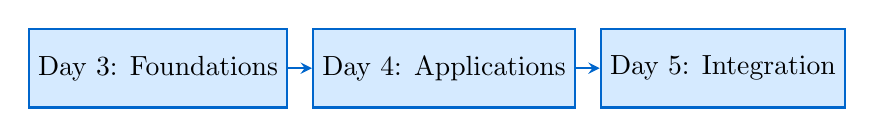
\begin{tikzpicture}
\node[process, minimum width=2.5cm] (d3) {Day 3: Foundations};
\node[process, minimum width=2.5cm, right=0.3cm of d3] (d4) {Day 4: Applications};
\node[process, minimum width=2.5cm, right=0.3cm of d4] (d5) {Day 5: Integration};

\draw[arrow] (d3) -- (d4);
\draw[arrow] (d4) -- (d5);
\end{tikzpicture}
\end{center}
\end{frame}

\end{document}
